\documentclass{beamer}
\usepackage[utf8]{inputenc}
\usepackage{amsmath,amssymb,amsthm,amsfonts}
\usepackage{graphicx}
\usepackage{booktabs}  % for table styling
\usepackage{bm}        % bold math symbols
\usepackage{algorithm}
\usepackage[noend]{algpseudocode}

\usepackage{adjustbox}
\usepackage{caption}
\usepackage{subcaption}

\usepackage{tikz}

\usepackage{settings}


% Title details
\title[CS Seminar / Hybrid Bit Recovery for LWE]{Cool and Cruel Bit Recovery Attack on LWE}
\subtitle{Sparse Binary Secrets and Partial Lattice Reduction}
\author[Mamanchuk Mykola]{\textbf{MAMANCHUK Mykola, SID.202420671} \\ \textbf{Supervising Professor: KUNIHIRO Noboru}}
\institute[UoT, CRISEC]{University of Tsukuba \\ Cryptography and Information Security Laboratory}
\date{\today}

% Section page template for better visual organization
\setbeamertemplate{section page}
{
  \begin{centering}
    \vspace{2cm}
    \usebeamercolor[fg]{section title}
    \usebeamerfont{section title}
    \insertsectionhead\par
    \vspace{0.5cm}
    \usebeamerfont{section title}
    Section \insertsectionnumber\par
  \end{centering}
}

% Optional: Subsection page template (if you use subsections)
\setbeamertemplate{subsection page}
{
  \begin{centering}
    \vspace{2cm}
    \usebeamerfont{subsection title}
    \insertsectionhead\par
    \usebeamerfont{subsection title}
    Subsection \insertsubsectionnumber: \insertsubsection\par
  \end{centering}
}

% Optional: Customize navigation symbols (if distracting)
\setbeamertemplate{navigation symbols}{}
\begin{document}

% ----------------------------------------------------------------------------
% TITLE SLIDE
% ----------------------------------------------------------------------------
\begin{frame}
  \titlepage
\end{frame}

% ----------------------------------------------------------------------------
% TABLE OF CONTENTS
% ----------------------------------------------------------------------------
\begin{frame}{Outline}
  \tableofcontents
\end{frame}

% ----------------------------------------------------------------------------
\section{Introduction}
% ----------------------------------------------------------------------------
\begin{frame}{Motivation \& Background}
  \textbf{Learning With Errors (LWE)} is a core problem in lattice-based cryptography,
  widely used in post-quantum cryptography (PQC).

  \vspace{0.4cm}
  \begin{itemize}
    \item \textbf{Sparse binary secrets}: e.g., $\mathbf{s} \in \{0,1\}^n$ with small Hamming weight $h$.
    \item \textbf{Homomorphic Encryption (HE)}: Often assumes small error and sparse secrets for efficiency.
    \item Traditional attacks do \emph{not} always account for these ``special'' parameters.
  \end{itemize}

  \vspace{0.4cm}
  \textbf{Key Challenge}: Evaluate real-world security of LWE with such specialized parameters.
\end{frame}

% ----------------------------------------------------------------------------
\begin{frame}{LWE Definition}
  \textbf{Search-LWE Problem:}

  \[
    \text{Given } \mathbf{A} \in \mathbb{Z}_q^{m \times n}, \quad
    \mathbf{b} = \mathbf{A} \cdot \mathbf{s} + \mathbf{e} \pmod{q},
  \]
  where
  \begin{itemize}
    \item $\mathbf{s} \in \mathbb{Z}_q^n$ is the secret vector,
    \item $\mathbf{e} \in \mathbb{Z}_q^m$ is the error (small-norm distribution),
    \item $m$ is the number of samples, $n$ is dimension, $q$ is a modulus.
  \end{itemize}

  \textbf{Goal}: Recover $\mathbf{s}$ given $\mathbf{A}$ and $\mathbf{b}$.

  \vspace{0.3cm}
  \textbf{Sparse Binary Setting}:
  \[
    \mathbf{s} \in \{0,1\}^n, \quad \text{Hamming weight } = h \ll n.
  \]
\end{frame}

% ----------------------------------------------------------------------------
\section{Core Idea of the Attack}
% ----------------------------------------------------------------------------
\begin{frame}{``Cool and Cruel'' Attack Overview}
  \textbf{Motivation}:
  \begin{itemize}
    \item Perform partial lattice reduction to separate LWE secret bits into:
    \begin{itemize}
      \item \textbf{Cruel bits}: Unreduced, high-variance portion
      \item \textbf{Cool bits}: Reduced, low-variance portion
    \end{itemize}
    \item Brute force the small ``cruel'' portion and then recover the ``cool'' part easily.
  \end{itemize}

  \vspace{0.4cm}
  \textbf{Three-Stage Attack}:
  \begin{enumerate}
    \item Parallel \emph{partial} lattice reduction,
    \item Brute force the ``cruel'' bits,
    \item Statistically recover the ``cool'' bits.
  \end{enumerate}
\end{frame}

% ----------------------------------------------------------------------------
\begin{frame}{Partial Lattice Reduction: Embedding}
  Consider the $(m+n)\times(m+n)$ matrix
  \[
    \Lambda =
    \begin{pmatrix}
       0      & qI_n \\
       \omega I_m & \mathbf{A}
    \end{pmatrix}.
  \]
  \begin{itemize}
    \item $\omega$ = penalty parameter controlling the trade-off
      between \emph{reduction quality} and \emph{error amplification}.
    \item Apply a lattice reduction algorithm (e.g., BKZ, ``flatter'').
  \end{itemize}

  \vspace{0.5cm}
  After reduction,
  \[
    \mathbf{A} \quad \longrightarrow \quad \mathbf{R}\mathbf{A} \equiv \mathbf{A}'.
  \]
  The first $n_u$ columns typically remain high-variance, the last $n_r = n-n_u$ are significantly reduced.
\end{frame}

% ----------------------------------------------------------------------------
\begin{frame}{Cruel vs. Cool Bits}
  \textbf{Cruel bits}:
  \begin{itemize}
    \item The $n_u$ unreduced columns (remain $\sim$uniform in $\mathbb{Z}_q$).
    \item Hard portion of the secret.
  \end{itemize}

  \textbf{Cool bits}:
  \begin{itemize}
    \item The $n_r = n - n_u$ reduced columns (low variance).
    \item Easy portion of the secret (recoverable with simple stats).
  \end{itemize}

  \vspace{0.3cm}
  \textbf{Key Observation}: 
  After partial reduction, the dot product $\mathbf{a}\cdot \mathbf{s}$ is dominated by
  the cruel bits if you guess them incorrectly. The correct guess yields a recognizable residual pattern, making it statistically distinguishable.
\end{frame}

% ----------------------------------------------------------------------------
\begin{frame}{Figure: Variance Separation}
  \begin{center}
    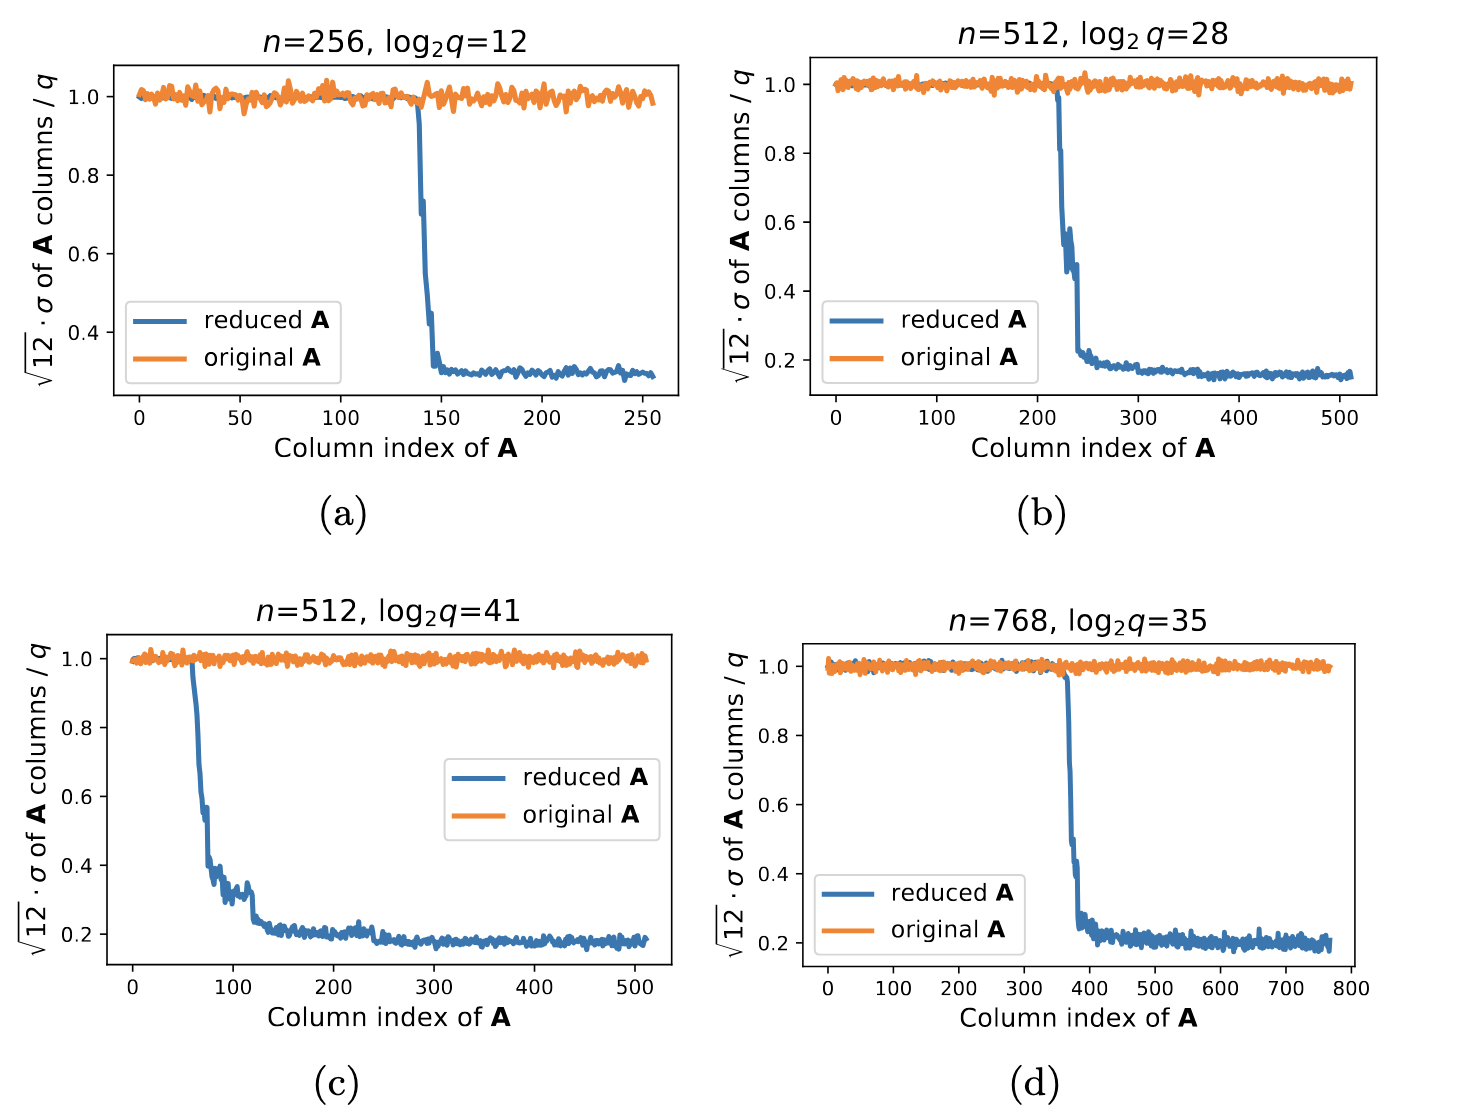
\includegraphics[width=0.7\linewidth]{example_variance_plot.png}
  \end{center}

  \scriptsize{
  \textbf{Conceptual Plot:}  
  The original $\mathbf{A}$ (orange) has uniform column variance $\approx q/\sqrt{12}$,
  while the reduced $\mathbf{A}'$ (blue) shows a significant drop after column index $n_u$.
  }
\end{frame}

% ----------------------------------------------------------------------------
\begin{frame}{Cruel Bit Brute Force}
  \textbf{Step 2 of Attack:}
  \begin{itemize}
    \item We only guess $\mathbf{s}_{0:n_u}$, the cruel portion.
    \item Evaluate
      \[
        \mathbf{R}\mathbf{A} \cdot \mathbf{s}^* - \mathbf{R}\mathbf{b} \pmod{q}
      \]
      for each guess $\mathbf{s}^*$ in that subspace.
    \item The \emph{correct guess} exhibits narrower standard deviation or a distinct residual distribution (as shown in next figure).
  \end{itemize}

  \vspace{0.4cm}
  \textbf{Why feasible?}  
  $n_u$ is significantly smaller than $n$; or the attacker knows $h_u$ (the smaller Hamming weight among the cruel bits).
\end{frame}

% ----------------------------------------------------------------------------
\begin{frame}{Figure: Residual Histograms}
  \begin{center}
    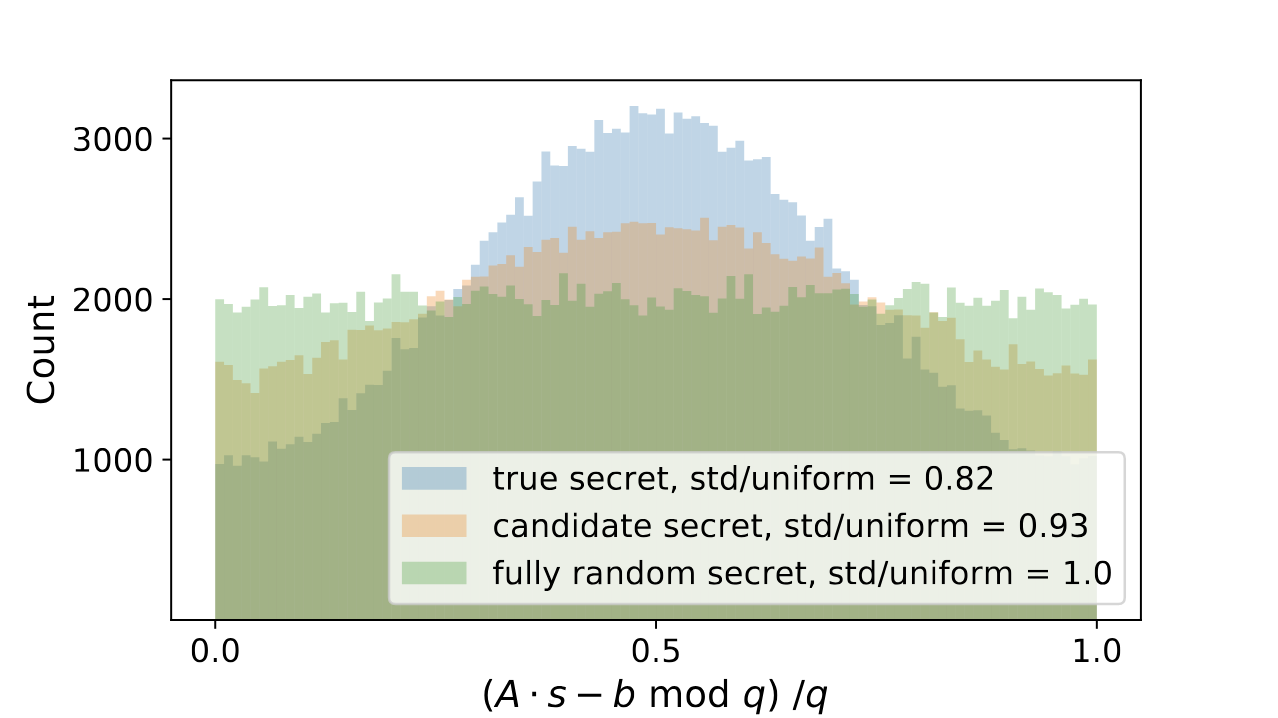
\includegraphics[width=0.65\linewidth]{residual_histogram.png}
  \end{center}

  \scriptsize{
  \textbf{Blue:} true secret residual distribution,  
  \textbf{Orange:} partial-correct guess (cruel bits correct),  
  \textbf{Green:} random guess.  
  Notice how the orange \& green differ in standard deviation or shape.
  }
\end{frame}

% ----------------------------------------------------------------------------
\begin{frame}{Cool Bit Recovery}
  After correctly identifying the $n_u$ cruel bits:

  \begin{itemize}
    \item The last $n_r$ columns are of \emph{low variance}.
    \item We can fix $\mathbf{s}_{0:n_u}$ and search each cool bit individually.
  \end{itemize}

  \textbf{Greedy Recovery (Algorithm 1):}
  \begin{itemize}
    \item For $i$ in $n - n_r : n$, flip bit $i$ and check standard deviation
      \[
        \sigma\bigl( (\mathbf{A}\mathbf{s}^* - \mathbf{b}) \bigr).
      \]
    \item Keep the bit flip if it \emph{lowers} or does not raise $\sigma$ significantly.
    \item Move on to the next bit.
  \end{itemize}
\end{frame}

% ----------------------------------------------------------------------------
\begin{frame}[fragile]{Algorithm 1: Greedy Recovery of Cool Bits}
\footnotesize
\begin{algorithm}[H]
\caption{Greedy Recovery of Cool Bits}
\begin{algorithmic}[1]
\Require $s^*$ initialized with correct cruel bits (size $n_u$) and 0 for $n_r$ bits
\For{$i \in \{n - n_r, \dots, n-1\}$}
  \State $s^*[i] \gets 0$
  \State $\sigma_0 \gets \sigma(\mathbf{A}\cdot s^* - \mathbf{b} \mod q)$
  \State $s^*[i] \gets 1$
  \State $\sigma_1 \gets \sigma(\mathbf{A}\cdot s^* - \mathbf{b} \mod q)$
  \If{$\sigma_0 \le \sigma_1$}
    \State $s^*[i] \gets 0$
  \Else
    \State $s^*[i] \gets 1$
  \EndIf
\EndFor
\end{algorithmic}
\end{algorithm}

\vspace{0.2cm}
\textbf{Idea}: flip each bit individually and choose the value that \emph{minimizes} the residual's standard deviation.
\end{frame}

% ----------------------------------------------------------------------------
\section{Complexities \& Results}
% ----------------------------------------------------------------------------
\begin{frame}{Complexities \& Experimental Timings}
  \textbf{Three Main Costs}:
  \begin{enumerate}
    \item \textbf{Lattice Reduction:} Performed in parallel (e.g., 12+ hours/matrix).
    \item \textbf{Brute Force on Cruel Bits:} Dependent on $n_u$ or $h_u$. (Often feasible if $n_u$ is small)
    \item \textbf{Statistical Recovery of Cool Bits:} Linear or near-linear in $n_r$.
  \end{enumerate}

  \vspace{0.2cm}
  \textbf{Reported Timings Example}:
  \begin{table}[h]
  \centering
  \scriptsize
  \begin{tabular}{cccc}
  \toprule
  $n$ & $\log_2 q$ & Hamming Weight & Time (seconds) \\
  \midrule
  256 & 12 & 12 & 3865 \\
  512 & 28 & 12 & 2417 \\
      & 41 & 60 & 376 \\
  768 & 35 & 12 & 1291 \\
  1024 & 50 & 17 & 6395 \\
  \bottomrule
  \end{tabular}
  \end{table}
\end{frame}

% ----------------------------------------------------------------------------
\begin{frame}{Why It Works}
  \begin{enumerate}
    \item \textbf{Non-uniform variance} after partial reduction splits the secret bits.
    \item \textbf{Statistical detection} of correct cruel bits via narrower distribution of residual.
    \item \textbf{Low-variance columns} let us do a simple one-bit-at-a-time approach for the cool bits.
  \end{enumerate}

  \vspace{0.3cm}
  \textbf{Practical Impact}:
  \begin{itemize}
    \item Sparse binary (and ternary) secrets are used in real cryptosystems (e.g., HE).
    \item This attack shows that certain parameter sets are vulnerable if $n_u$ is not too large and the penalty parameter is well-tuned.
  \end{itemize}
\end{frame}

% ----------------------------------------------------------------------------
\section{Attack Overview}
\subsection*{Conclusion}
% ----------------------------------------------------------------------------
\begin{frame}{Takeaways and Next Steps}
  \textbf{Key Points}:
  \begin{itemize}
    \item Partial lattice reduction $\rightarrow$ \textit{cruel vs. cool} separation.
    \item Brute force on a small subproblem, then linear-time statistical recovery.
    \item Attacks extended to RLWE for 2-power cyclotomic rings (rotation trick).
  \end{itemize}

  \vspace{0.3cm}
  \textbf{Ongoing \& Future Work}:
  \begin{itemize}
    \item Further optimization or alternative partial reduction for smaller overhead.
    \item Combine with other ML-based distinguishers (e.g., SALSA, transformers).
    \item Evaluate larger $n$ and different error/secret distributions (ternary, Gaussian).
  \end{itemize}
\end{frame}
% ----------------------------------------------------------------------------
\section{Practical Considerations}
% ----------------------------------------------------------------------------
\begin{frame}{Implementation \& Parallel Brute Force}
  \textbf{Key Points:}
  \begin{itemize}
    \item \textbf{Implementation Setup:}
      \begin{itemize}
        \item Written in Python, accelerated with \texttt{pytorch} on GPUs.
        \item Batches of secret candidates evaluated in parallel.
      \end{itemize}
    \item \textbf{Brute Force for Cruel Bits:}
      \begin{itemize}
        \item Enumerate possible secret values for the ``cruel'' part of $\mathbf{s}$.
        \item Evaluate residuals $\mathbf{A}\mathbf{s}^* - \mathbf{b}$ mod $q$.
      \end{itemize}
    \item \textbf{Ascending Hamming Weight:}
      \begin{itemize}
        \item Start with Hamming weight 0, 1, 2, etc.
        \item Keep top-$k$ candidates for deeper evaluation.
      \end{itemize}
  \end{itemize}

  \vspace{0.3cm}
  \textbf{Parallelizability:}  
  Because each candidate check is independent, the brute force step scales linearly with the number of GPUs/cores.
\end{frame}

% ----------------------------------------------------------------------------
\begin{frame}{Candidate Evaluation: Variance Test}
  \textbf{Residual Distribution:}
  \[
    x \;=\; \mathbf{A}\mathbf{s}^* - \mathbf{b} \pmod{q}.
  \]
  \begin{itemize}
    \item If $\mathbf{s}^*$ is \emph{wrong} (cruel bits incorrect) $\implies x \approx \text{uniform}$ mod $q$.
    \item If $\mathbf{s}^*$ is \emph{correct} (for the cruel portion) $\implies x$ has smaller variance, akin to a ``mod-Gaussian.''
  \end{itemize}

  \vspace{0.3cm}
  \textbf{Why Variance?}
  \begin{itemize}
    \item Non-parametric tests (K-S, Kuiper) can be slow on large $N$.
    \item Likelihood tests over modulo Gaussians require summations over $k\cdot q$ shifts.
    \item \textbf{Simple approach}: compute sample variance $\hat{\sigma}^2(x)$ and compare to known threshold(s).
  \end{itemize}
\end{frame}

% ----------------------------------------------------------------------------
\begin{frame}{GPU Implementation Details}
  \textbf{Precision Considerations:}
  \begin{itemize}
    \item $q$ can be large (e.g., $\log_2 q$ up to 50).
    \item Scaling data down for 16-bit floats is sufficient because we only need relative variance info.
  \end{itemize}

  \vspace{0.3cm}
  \textbf{PyTorch Compilation:}
  \begin{itemize}
    \item Just-In-Time or graph-based optimization yields $2\text{-}3\times$ speedup vs. eager mode.
  \end{itemize}

  \vspace{0.3cm}
  \textbf{Throughput Example:}
  \begin{itemize}
    \item On one NVIDIA V100, $\sim5$ billion secret candidates ($n=512$) tested in $\approx1$ hour.
    \item Bruteforce is repeated until the correct guess emerges (with high probability).
  \end{itemize}
\end{frame}

% ----------------------------------------------------------------------------
\section{Lattice Reduction}
% ----------------------------------------------------------------------------
\begin{frame}{Need for Partial Lattice Reduction}
  \textbf{Recall Attack Flow:}
  \begin{enumerate}
    \item \emph{Reduce} an embedded matrix $\Lambda$ to obtain new $(\mathbf{A}', \mathbf{b}')$ with column variance partially compressed.
    \item Identify high-variance columns (cruel) vs. low-variance columns (cool).
    \item Brute force on cruel bits, then linear-time fix of cool bits.
  \end{enumerate}

  \textbf{Why partial?}
  \begin{itemize}
    \item Overly strong reduction $\implies$ massive noise amplification, complicating distribution tests.
    \item Too weak reduction $\implies$ not enough columns are reduced (large $n_u$).
  \end{itemize}
\end{frame}

% ----------------------------------------------------------------------------
\begin{frame}{Generating Enough Reduced LWE Data}
  \textbf{Sub-Sampling:}
  \begin{itemize}
    \item If you start with $m_0$ LWE samples, choose subsets of size $m_1$ repeatedly.
    \item Each subset forms a new $(m_1 + n)\times(m_1 + n)$ $q$-ary lattice for reduction.
    \item This \textbf{inflates} the total number of partially reduced data sets, crucial when $m$ is small.
  \end{itemize}

  \vspace{0.3cm}
  \textbf{SALSA Picante \cite{SALSAref}:}
  \begin{itemize}
    \item Eavesdropped $4n$ samples, sub-sampled $n$ at a time for repeated BKZ runs.
    \item \emph{This paper} uses $m = \mathrm{round}(0.875\,n)$ from $4n$ total.
  \end{itemize}

  \vspace{0.3cm}
  \textbf{Conclusion:}
  \begin{itemize}
    \item Each sub-lattice reduced $\implies$ yields a distinct reduced matrix $\mathbf{A}'$.
    \item Attack = gather many $\mathbf{A}'$'s for large-scale statistical checks.
  \end{itemize}
\end{frame}

% ----------------------------------------------------------------------------
\begin{frame}{Choice of Reduction Algorithms}
  \textbf{Three Tools}:
  \begin{enumerate}
    \item BKZ2.0 \cite{BKZ2ref}: strong reduction but slow for big block sizes/dimensions.
    \item flatter \cite{FlatterRef}: fast for $n \ge 512$ and large $q$, but might get stuck.
    \item polish \cite{PolishRef}: final orthogonalization step after flatter or BKZ.
  \end{enumerate}

  \vspace{0.3cm}
  \textbf{Measuring Performance:}  
  \[
    \rho = \frac{\sigma(\mathbf{A}')}{\sigma(\mathbf{A}_{\text{initial}})} \quad \text{with} \quad
    \sigma(\mathbf{A}_{\text{initial}}) = \frac{q}{\sqrt{12}}.
  \]
  \begin{itemize}
    \item $\rho \ll 1 \implies$ large norm reduction.
    \item Attack wants $\rho$ small but not so small that noise becomes unmanageable.
  \end{itemize}
\end{frame}

% ----------------------------------------------------------------------------
\begin{frame}{Interleaving \& Early Termination}
  \textbf{Interleaving BKZ \& flatter}:
  \begin{itemize}
    \item Run flatter for a few rounds.
    \item If average $\Delta\rho < 0.001$ over 3 iters, switch to BKZ2.0.
    \item After BKZ, run polish, then switch back to flatter, etc.
  \end{itemize}

  \textbf{Early Termination}:
  \begin{itemize}
    \item Once $\rho$ stalls or improvements become tiny, export the reduced matrix $\mathbf{A}'$.
    \item Sub-sample a new set of LWE samples, repeat fresh.
    \item Maximizes the number of distinct partially reduced data sets from one heavy reduction session.
  \end{itemize}
\end{frame}

% ----------------------------------------------------------------------------
\begin{frame}{Result: Cruel Bits $\approx \rho^2 n$}
  \begin{itemize}
    \item Empirically, $n_u \approx \rho^2 \, n$.
    \item Fewer cruel bits $\implies$ smaller dimension for brute force.
    \item If $\rho^2 n$ is still large, brute force is more expensive.
  \end{itemize}

  \vspace{0.4cm}
  \textbf{Trade-off Recap}:
  \begin{itemize}
    \item $\omega$ (penalty param) and choice of algorithms $\implies$ final $\rho$.
    \item Must keep error amplification from $|\mathbf{R}\mathbf{e}|$ under control, or distributions become too wide to distinguish.
  \end{itemize}
\end{frame}

% ----------------------------------------------------------------------------
\section{Statistical Tests}
% ----------------------------------------------------------------------------
\begin{frame}{Cruel Bit Verification: Sample Complexity}
  \textbf{Distinguishing Uniform vs. Mod-Gaussian:}
  \[
    x = \mathbf{a}\cdot(s^* - s) - e \pmod{q}.
  \]
  \begin{itemize}
    \item If $s^*$ has correct cruel bits, $x$ has smaller variance $\sigma_{G_q}^2$.
    \item Otherwise, $x \approx \text{uniform}$ with variance $\sigma_{U_q}^2 \approx \frac{q^2}{12}\text{.}$  \end{itemize}

  \vspace{0.4cm}
  \textbf{Variance Test}:  
  For $M$ samples, 
  \[
    \hat{\sigma}^2 = \frac{1}{M}\sum x_i^2.
  \]

  \textbf{CLT-based Bound}:  
  \[
    M(\alpha, \beta) \approx
      \left[
        \frac{\,G^{-1}(\alpha)\,\sigma_{U_q^2} + G^{-1}(\beta)\,\sigma_{G_q^2}\,}
             {\sigma_{G_q}^2 - \sigma_{U_q}^2}
      \right]^2,
  \]
  controlling false negative $\alpha$ and false positive $\beta$ errors.
\end{frame}

% ----------------------------------------------------------------------------
\begin{frame}{Concrete $M$ Values (Table 5)}
  \begin{center}
    \scriptsize
    \begin{tabular}{cccccc}
    \toprule
    $n$ & $\log_2 q$ & $n_u$ & $h$ & Worst Case $M$ & Avg Case $M$ \\
    \midrule
    256 & 12 & 143 & 12 & $5.67\times10^4$ & $1.12\times10^4$ \\
    512 & 28 & 228 & 20 & $3.29\times10^3$ & $1.66\times10^3$ \\
    512 & 41 & 75  & 60 & $1.98\times10^4$ & $1.02\times10^4$ \\
    768 & 35 & 373 & 20 & $3.13\times10^4$ & $9.74\times10^3$ \\
    768 & 35 & 373 & 64 & $6.21\times10^6$ & $1.47\times10^5$ \\
    1024 & 50 & 495 & 15 & $2.37\times10^3$ & $1.35\times10^3$ \\
    \bottomrule
    \end{tabular}
  \end{center}

  \vspace{0.2cm}
  \scriptsize{
    \textbf{Note:}
    - Worst case: all secret 1-bits in reduced region.  
    - Average case: 1-bits split proportionally.  
    - $M$ can be as low as a few thousand samples for some parameters or up to $10^6$ for tough scenarios.
  }
\end{frame}

% ----------------------------------------------------------------------------
\begin{frame}{5.2 Testing Cool Bit Predictions}
  \textbf{Algorithm 1 (Greedy) Recap}:  
  \begin{itemize}
    \item Flip each cool bit $k$ from 0 to 1,
      measure $\hat{\sigma}^2(x_1)$ vs. $\hat{\sigma}^2(x_0)$.
    \item Keep the value that yields smaller residual variance.
  \end{itemize}

  \textbf{Statistically:}
  \[
    \delta(\sigma^2) = \hat{\sigma}^2(x_1) - \hat{\sigma}^2(x_0).
  \]
  \begin{itemize}
    \item If bit $k$ truly $=1$, setting it to 1 \emph{reduces} the variance in the presence of the correct preceding bits.
    \item Otherwise, it \emph{increases} or doesn't lower variance enough, so keep it at 0.
  \end{itemize}
\end{frame}

% ----------------------------------------------------------------------------
\section{Attack Performance}
% ----------------------------------------------------------------------------
\begin{frame}{Overall Results \& Timings}
  \textbf{Key Steps:}
  \begin{enumerate}
    \item Lattice reduction (parallel): hours-scale for large $n$, but done once to generate multiple sub-samples.
    \item Brute force on $n_u$ cruel bits: total time depends on how quickly the correct candidate is found in ascending Hamming weight.
    \item Cool bits: linear time via the greedy approach.
  \end{enumerate}

  \vspace{0.4cm}
  \textbf{Table 6 (example)}:
  \begin{itemize}
    \item For $n=512,\; \log_2 q=41,\; h=60$:
      \begin{itemize}
        \item $\approx 6$ minutes on 1 GPU for secret recovery (excluding lattice reduction).
        \item Lattice reduction itself might take 12 hours/matrix but is fully parallelizable.
      \end{itemize}
    \item Larger $n=768$ or $1024$ also feasible with multi-GPU setups.
  \end{itemize}
\end{frame}

% ----------------------------------------------------------------------------
\section{Conclusions}
\begin{frame}{Keynotes for Implementation and Performance}
  \begin{itemize}
    \item \textbf{Parallel Sub-Sampling:}
      \begin{itemize}
        \item Increases number of reduced matrices from limited $m_0$ LWE samples.
        \item More reduced data = easier distribution testing.
      \end{itemize}
    \item \textbf{Partial Lattice Reduction:}
      \begin{itemize}
        \item Balanced by penalty $\omega$ and the interleaving approach (BKZ + flatter).
        \item Achieves a sweet spot with $\rho \ll 1$ but not too large error amplification.
      \end{itemize}
    \item \textbf{Cruel vs. Cool Recovery:}
      \begin{itemize}
        \item Brute force the small subset $n_u\approx \rho^2 n$, detect correctness by variance.
        \item Greedy fix the remaining $n_r$ bits.
      \end{itemize}
    \item \textbf{Efficient Implementation:}
      \begin{itemize}
        \item GPU parallelization + simple variance test.
        \item Feasible for $n \le 1024$ even with high Hamming weight.
      \end{itemize}
  \end{itemize}
\end{frame}

\section{Recovery Results}
% ----------------------------------------------------------------------------
\begin{frame}{Concrete Performance Results}
  \textbf{Overview (Refer to Table 6 \cite{concrete_results})}:
  \begin{itemize}
    \item After partial lattice reduction (Section~4), the main cost is enumerating over the ``cruel'' bits in ascending Hamming weight.
    \item We periodically apply the greedy approach (Algorithm 1) to recover the cool bits, e.g., every 40M secret candidates.
    \item Timing includes:
      \begin{itemize}
        \item $\sim 10$ seconds of JIT compilation,
        \item $\sim 10$ seconds of data loading,
        \item GPU-based parallel brute force for the cruel portion.
      \end{itemize}
  \end{itemize}

  \vspace{0.3cm}
  \textbf{Notes on Hamming Weights}:
  \begin{itemize}
    \item Higher $h$ $\implies$ typically more enumeration, or bigger chance $h_u$ is large.
    \item Attackers can rely on multi-GPU setups (e.g., up to 20 GPUs for the toughest cases).
  \end{itemize}
\end{frame}

% ----------------------------------------------------------------------------
\begin{frame}{Table 6 \cite{concrete_results}: Examples}
  \footnotesize
  \begin{itemize}
    \item The table shows dimension $n$, $\log_2 q$, secret Hamming weight $h$, the number of bits in the cruel part $h_u$, and the fraction of secrets that produce that $h_u$ (for random secrets).
    \item \textbf{Time (Min/Max)} depends on when the correct partial secret guess is found in the ascending-Hamming order.
    \item Typical sample usage: 200k for brute force, 1M for the greedy step at higher $h$ settings.
  \end{itemize}

  \vspace{0.2cm}
  \textbf{Highlights}:
  \begin{itemize}
    \item For $n=256,\;\log_2 q=12,\;h=12$, some guesses complete in tens of seconds, while higher $h_u$ can take thousands of seconds.
    \item $n=512,\;\log_2 q=41,\;h=60$ may finish in a few hundred seconds for certain $h_u$ but potentially longer for others.
  \end{itemize}
  \vspace{0.3cm}

  \textbf{Key Takeaway}: 
  \begin{itemize}
    \item The final recovery time strongly correlates with $h_u$ (the 1-bits inside the cruel region). 
    \item If $h_u$ is small, the enumeration search is drastically faster.
  \end{itemize}
\end{frame}

% ----------------------------------------------------------------------------
\subsection{Comparison with Existing Attacks}
% ----------------------------------------------------------------------------
\begin{frame}{Comparisons to Hybrid Dual MiTM, etc.}
  \textbf{Why compare?}
  \begin{itemize}
    \item The hybrid dual meet-in-the-middle (MiTM) approach \cite{ref_mitm} is conceptually closest.
    \item Some references \cite{ref_smalln}, \cite{ref_largen} provide partial results but mostly for $n<110$ or smaller $\log q$.
  \end{itemize}

  \vspace{0.3cm}
  \textbf{Table~\ref{tab:comparison_results}}:
  \begin{itemize}
    \item Shows the LWE Estimator predictions (ROP = number of ring ops).
    \item Compares them to actual code from \cite{ref_sparse} which times out or fails at $n>256$.
    \item Our “Cool and Cruel” approach does scale to $n=768$, $n=1024$ with feasible timings.
  \end{itemize}

  \vspace{0.3cm}
  \textbf{Conclusion}:
  \begin{itemize}
    \item Estimator-based ROP metrics can underestimate the real cost or do not translate well to GPU times.
    \item Actual meet-in-the-middle code \cite{ref_sparse} does not succeed beyond $n=256$ in multi-week runs.
  \end{itemize}
\end{frame}

% ----------------------------------------------------------------------------
\subsection{2-power Cyclotomic Ring-LWE}
% ----------------------------------------------------------------------------
\begin{frame}{RLWE Basics}
  \textbf{Ring-LWE Setting}:
  \begin{itemize}
    \item $R_q = \mathbb{Z}_q[x]/(x^n+1)$ with $n=2^k$.
    \item RLWE sample: $(\,a(x),\; b(x) = a(x)\cdot s(x)+e(x)\,)$
          corresponds to a skew-circulant matrix $A_{\text{circ}}$.
    \item Some RLWE rings can be attacked more easily than generic LWE \cite{someRLWEref}, but 2-power cyclotomic rings remain a NIST standard candidate.
  \end{itemize}

  \vspace{0.3cm}
  \textbf{Our Attack}:
  \begin{itemize}
    \item After partial reduction, columns still separate into cruel vs. cool.
    \item \textbf{Crucial difference:} We can rotate (shift) the cruel region across the ring polynomial, effectively searching multiple windows of length $n_u$.
  \end{itemize}
\end{frame}

% ----------------------------------------------------------------------------
\begin{frame}{Figure: LWE vs. RLWE Cost Ratio}
  \begin{center}
    % Adjust the filename to match your actual image file
    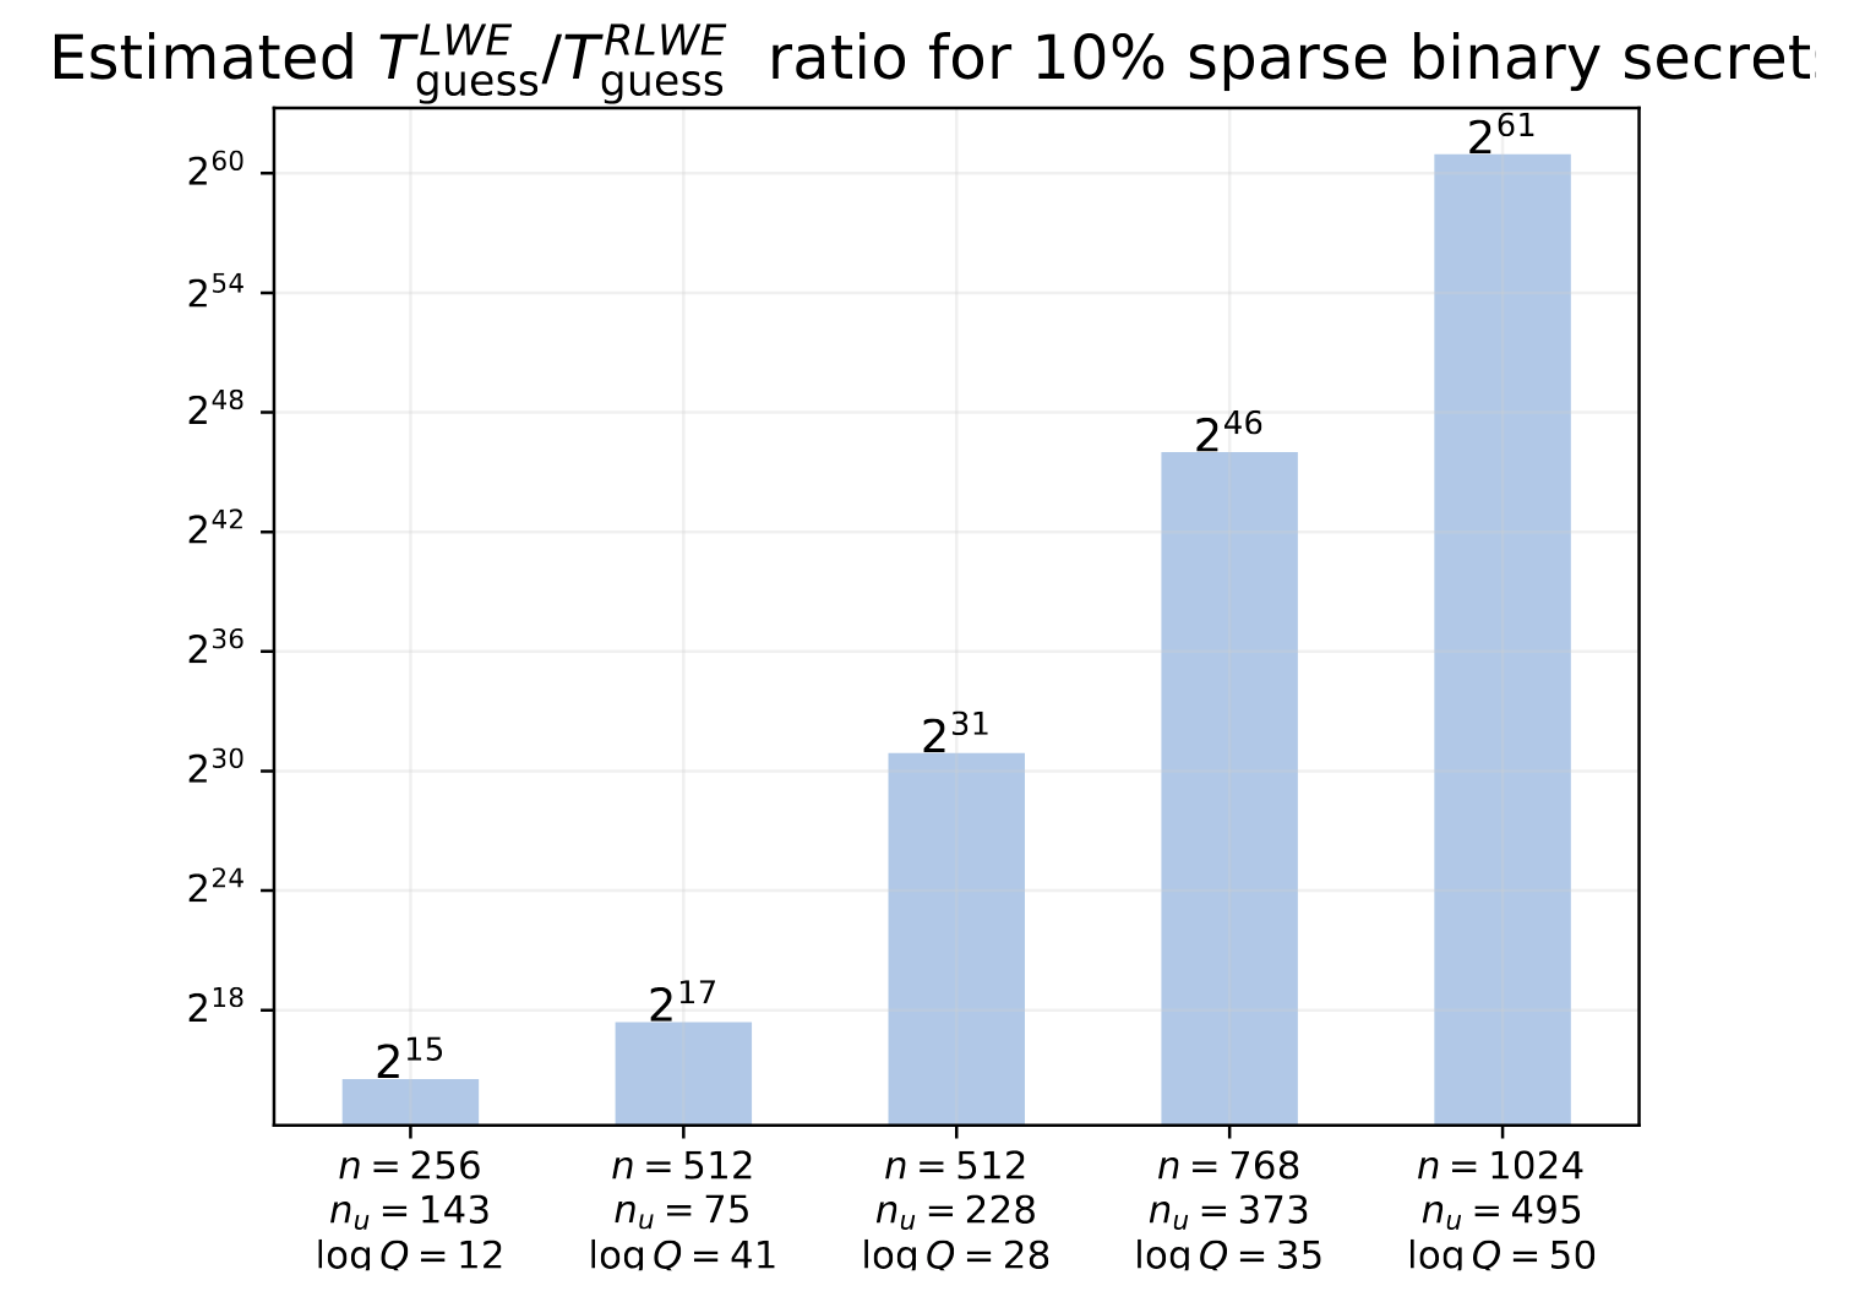
\includegraphics[width=0.7\linewidth]{rlwe_lwe_ratio.png}
  \end{center}
  \scriptsize{
  \textbf{Fig.3 Example:} \,
  Attack cost ratio $T^{\text{LWE}}_{\text{guess}} / T^{\text{RLWE}}_{\text{guess}}$ for 10\% sparse binary secret, shown for $(n=256,\;512,\;768,\;1024)$. 
  Notice the exponential differences (e.g. $2^{31}, 2^{46}, 2^{61}$) as dimension grows.
  }
\end{frame}

% ----------------------------------------------------------------------------
\begin{frame}{RLWE Cruel Bit Shifting}
  \textbf{Key Technique}:
  \begin{itemize}
    \item We can shift the matrix $A$ or the polynomial $a(x)$ so that different subsets of the secret $s$ fall into the first $n_u$ columns.
    \item Let $h_{n_u,i}(s)$ = \# of 1-bits in $s$ over a length-$n_u$ window starting at index $i$.
    \item We define $h_u^{(1)}(s) = \min_{0\le i<n}h_{n_u,i}(s)$, the minimal number of 1s in \emph{any} length-$n_u$ window.
  \end{itemize}

  \vspace{0.2cm}
  \textbf{Why Faster?}
  \begin{itemize}
    \item If $h_u^{(1)}(s) \ll h_u(s)$, the enumerations become smaller by orders of magnitude.
    \item Potentially run $n$ windows in parallel or pick the best (lowest-weight) window for brute force.
  \end{itemize}
\end{frame}

% ----------------------------------------------------------------------------
\begin{frame}{Table 8 Example: $(n=256,\;\log_2 q=12,\;h=12)$}
  \footnotesize
  \begin{itemize}
    \item Each row: a secret with $h_u(s)$ cruel bits (LWE viewpoint) vs. $h_u^{(1)}(s)$ after ring shifts.
    \item LWE times blow up quickly for large $h_u(s)$, sometimes not finishing (indicated by ``--'').
    \item RLWE approach can exploit smaller $h_u^{(1)}$ windows, finishing in $10^3$ or $10^4$ seconds.
  \end{itemize}

  \vspace{0.2cm}
  \textbf{Findings}:
  \begin{itemize}
    \item RLWE times $\approx 10^3\times$ or more faster on average than LWE if ring shifting reveals a sufficiently small subset of bits.
    \item Estimated vs. actual times differ but confirm a wide gap in many tested secrets.
  \end{itemize}
\end{frame}

% ----------------------------------------------------------------------------
\begin{frame}{Table 9 Example: $(n=512,\;\log_2 q=41,\;h=60)$}
  \footnotesize
  \begin{itemize}
    \item Similar structure: 10 random secrets, each with a certain $h_u(s)$ for LWE and minimal $h_u^{(1)}(s)$ for RLWE.
    \item For large $h_u(s)$, the LWE brute force can be impractical, while RLWE shifting might find a window with only 3--5 bits.
  \end{itemize}
  \vspace{0.2cm}
  \textbf{Key Observations}:
  \begin{itemize}
    \item Some secrets never complete under LWE enumeration (`--`), but RLWE recovers them due to partial shifting.
    \item The measured time can be $10^4$ or $10^5$ sec, significantly lower than the naive $10^7$ or $10^9$ sec if no shift is used.
  \end{itemize}
\end{frame}

% ----------------------------------------------------------------------------
\begin{frame}{RLWE vs. LWE: Overall Implications}
  \begin{itemize}
    \item The ability to rotate the secret in $2$-power cyclotomic RLWE leads to a \textbf{big advantage} for the attacker if the secret is sparse.
    \item In practice, partial lattice reduction cost is roughly the same, so the big gain is purely from enumerating fewer 1-bits in the cruel region.
    \item For real homomorphic encryption or ring-based cryptography, adopting small/sparse secrets can be \emph{riskier} than previously assumed.
  \end{itemize}

  \vspace{0.3cm}
  \textbf{High-Level Conclusion}:
  \begin{itemize}
    \item For $n=256, 512, 1024$, the empirical data (Tables 8--9, Figure 3) confirm that ``Cool and Cruel'' attacks on RLWE can be up to $10^3$--$10^5$ times faster compared to a standard LWE scenario with the same dimension/modulus.
  \end{itemize}
\end{frame}

% --------------------------------------------------------------------------
% DISCUSSION AND FUTURE WORK
% --------------------------------------------------------------------------
\section{Discussion and Future Work}

\begin{frame}{}
    \Huge \centering
    Further Objectives
\end{frame}

\begin{frame}{Summary of Main Findings}
  \textbf{Cool \& Cruel Attack Recap:}
  \begin{itemize}
    \item Partial Lattice Reduction splits secret bits into \textit{cruel} vs. \textit{cool}.
    \item GPU-based brute force on cruel bits, variance-based or greedy approaches for cool bits.
    \item Demonstrated practicality up to $n=1024$, especially for sparse secrets.
    \item RLWE (2-power cyclotomic) further lowers the dimension due to \emph{cruel bit shifting}.
  \end{itemize}

  \vspace{0.3cm}
  \textbf{Open Questions:}
  \begin{itemize}
    \item Large-scale brute force is still exponential.
    \item Lattice reduction vs. error amplification trade-off is not fully optimized.
    \item Sample-hungry approach for the cool bits remains a bottleneck when $\sigma_e$ is large.
  \end{itemize}
\end{frame}

% ----------------------------------------------------------------------------
\begin{frame}{1. Improving the Combinatorial Scaling}
  \textbf{Problem Statement:}
  \begin{itemize}
    \item After partial reduction, we brute force $n_u$ cruel bits. 
    \item If $n_u$ or the partial Hamming weight is large, enumeration can be very costly.
  \end{itemize}

  \textbf{Potential Solutions:}
  \begin{enumerate}
    \item \textbf{Meet-in-the-Middle (MiTM) / Hybrid Attacks:}
      \begin{itemize}
        \item Split $n_u$ bits into two halves, store partial sums, combine them to find matches.
        \item Reduces complexity from $2^{n_u}$ to $\sim 2^{n_u/2}$ with memory trade-offs.
      \end{itemize}
    \item \textbf{Heuristic Pruning or ML-Based Ranking:}
      \begin{itemize}
        \item E.g., a small neural net or logistic model to discard unlikely bit patterns quickly.
        \item Inspired by SALSA-type or other learning-based approaches.
      \end{itemize}
  \end{enumerate}
  
  \textbf{Approaches / Techniques:}
  \begin{itemize}
    \item Hashed partial sums, advanced data structures, GPU kernels for MiTM.
    \item Minimal overhead ``Early Abort'' style checks or distribution-based pruning.
  \end{itemize}
\end{frame}

% ----------------------------------------------------------------------------
\begin{frame}{2. Balancing Reduction and Secret Recovery}
  \textbf{Problem Statement:}
  \begin{itemize}
    \item Stronger lattice reduction $\rightarrow$ fewer cruel bits, but higher error amplification $\sigma_e$.
    \item We do not currently co-optimize the partial reduction depth with enumeration cost.
  \end{itemize}
  
  \textbf{Potential Solutions:}
  \begin{enumerate}
    \item \textbf{Adaptive / Incremental Approach:}
      \begin{itemize}
        \item Perform partial reduction in stages, attempt partial enumeration, then refine as needed.
      \end{itemize}
    \item \textbf{Search-Based Parameter Tuning:}
      \begin{itemize}
        \item Model the total cost $T(\omega) = T_{\mathrm{reduction}}(\omega) + T_{\mathrm{enum}}(\omega)$,
              find $\omega$ or blocksize $\beta$ that minimizes $T(\omega)$ in practice.
      \end{itemize}
  \end{enumerate}

  \textbf{Approaches / Techniques:}
  \begin{itemize}
    \item Heuristic optimization (simulated annealing, etc.), or real-time feedback on enumeration performance.
    \item Possibly do partial re-reduction of sub-lattices if the dimension is still too large.
  \end{itemize}
\end{frame}

% ----------------------------------------------------------------------------
\begin{frame}{3. Improving Cool Bit Recovery (Sample Efficiency)}
  \textbf{Problem Statement:}
  \begin{itemize}
    \item Current approach (Algorithm 1) flips each bit $\rightarrow$ measure variance 
      $\sigma(\mathbf{A}\,\mathbf{s}^* - \mathbf{b})$.
    \item If $\sigma_e$ is large, we may need many samples to distinguish flipping one bit at a time.
  \end{itemize}

  \textbf{Potential Solutions:}
  \begin{enumerate}
    \item \textbf{Machine Learning Distinguishers:}
      \begin{itemize}
        \item Train a small classifier to evaluate correct vs.\ incorrect bit patterns 
              without per-bit variance checks.
      \end{itemize}
    \item \textbf{Batch or Group Testing:}
      \begin{itemize}
        \item Flip multiple bits simultaneously, analyze changes. 
        \item Potentially reveal multiple bits in fewer samples.
      \end{itemize}
  \end{enumerate}
  
  \textbf{Approaches / Techniques:}
  \begin{itemize}
    \item Shallow neural networks or logistic regression for bit classification in reduced $\mathbf{A}'$.
    \item Carefully designed “group tests” (like combinatorial group testing) 
      with distribution difference metrics.
  \end{itemize}
\end{frame}

% ----------------------------------------------------------------------------
\begin{frame}{Additional Directions}
  \textbf{Beyond the Above:}
  \begin{itemize}
    \item \textbf{Ternary / Gaussian Secrets:} 
      Test if the partial-lattice method extends to other secret distributions used in practice.
    \item \textbf{Combining with SALSA or Transformers:}
      \begin{itemize}
        \item A synergy of partial reduction plus advanced ML might further reduce sample usage.
      \end{itemize}
    \item \textbf{Real-World Impact / Mitigations:}
      \begin{itemize}
        \item Evaluate big-name homomorphic encryption libraries to see if they inadvertently allow 
              small $h$ secrets or ring structures that are highly vulnerable.
      \end{itemize}
  \end{itemize}

  \vspace{0.3cm}
  \textbf{Conclusion}:
  \begin{itemize}
    \item \textbf{Cool \& Cruel} is already practical, but many improvements remain to push it further
          or to defend against it.
    \item Future research will likely refine each stage (reduction, brute force, final bit checks) 
          for greater efficiency.
  \end{itemize}
\end{frame}
% --------------------------------------------------------------------------
\section{Proposal: Cool, Chill, and Cruel}

\section{Discussion and Future Work}

\begin{frame}{}
    \centering {\Huge 
    Cool, Chill, and Cruel} \\
    Optimize for Potential Recovery
\end{frame}
% --------------------------------------------------------------------------

\begin{frame}{Motivation for Multi-Zone Approach}
\textbf{Motivation:} After partial lattice reduction, the standard deviation $\sigma(\mathbf{A}_{*,j})$ of columns
often does \emph{not} drop at a single index but rather transitions over a slope.
Thus, we propose dividing columns into:
\begin{itemize}
  \item \textbf{Cruel region} (green): High variance $\approx q/\sqrt{12}$.
  \item \textbf{Chill region} (yellow): Transitional/slope columns with moderate variance.
  \item \textbf{Cool region} (blue): Low variance, easily distinguished bits.
\end{itemize}

\textbf{Goal:} Use a \emph{specialized} algorithm in the Chill zone to reduce brute force cost on partially reduced columns,
while still using standard brute force for Cruel bits and a simple classification for fully Cool bits.

\vspace{0.3cm}
\textbf{Key Observations:}
\begin{itemize}
  \item The boundary between these regions is determined by variance thresholds (or slope detection).
  \item Each zone is handled with a \emph{tailored} approach (brute force, partial classification, or easy flips).
\end{itemize}
\end{frame}

% --------------------------------------------------------------------------
\begin{frame}{Annotated Figures: Cruel, Chill, and Cool Regions}
\begin{figure}[ht]
    \centering
    % Subfigure 1
    \begin{subfigure}{0.49\textwidth}
        \centering
        \begin{tikzpicture}
            \node[anchor=south west, inner sep=0] (image) at (0,0)
              {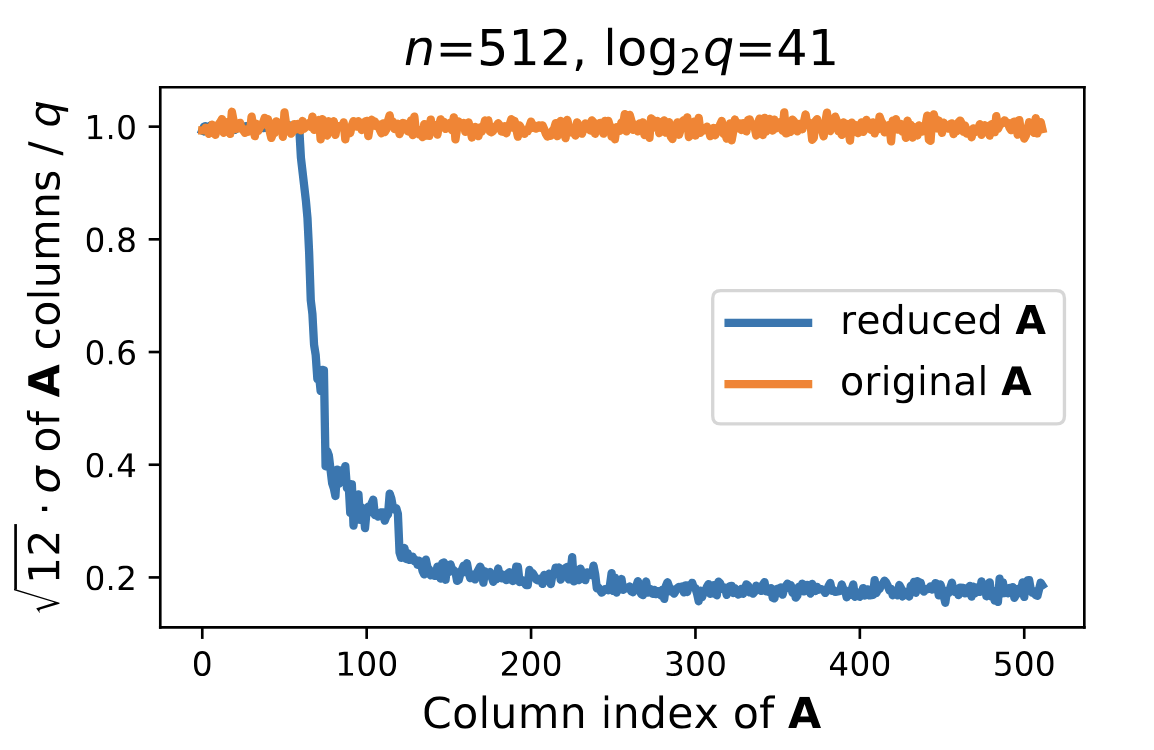
\includegraphics[width=\textwidth]{512-41.png}};
            \begin{scope}[x={(image.south east)}, y={(image.north west)}]
                % Cruel region (green frame)
                \draw[thick, green, fill=green!20, opacity=0.3] (0.18, 0.19) rectangle (0.28, 0.8);
                % Chill region (yellow frame)
                \draw[thick, yellow, fill=yellow!20, opacity=0.3] (0.285, 0.19) rectangle (0.345, 0.8);
                % Cool region (blue frame)
                \draw[thick, blue, fill=blue!20, opacity=0.3] (0.35, 0.19) rectangle (0.91, 0.8);
            \end{scope}
        \end{tikzpicture}
        \caption{\small $n=512,\,\log_2 q=41$.}
        \label{fig:region1}
    \end{subfigure}
    \hfill
    % Subfigure 2
    \begin{subfigure}{0.49\textwidth}
        \centering
        \begin{tikzpicture}
            \node[anchor=south west, inner sep=0] (image) at (0,0)
              {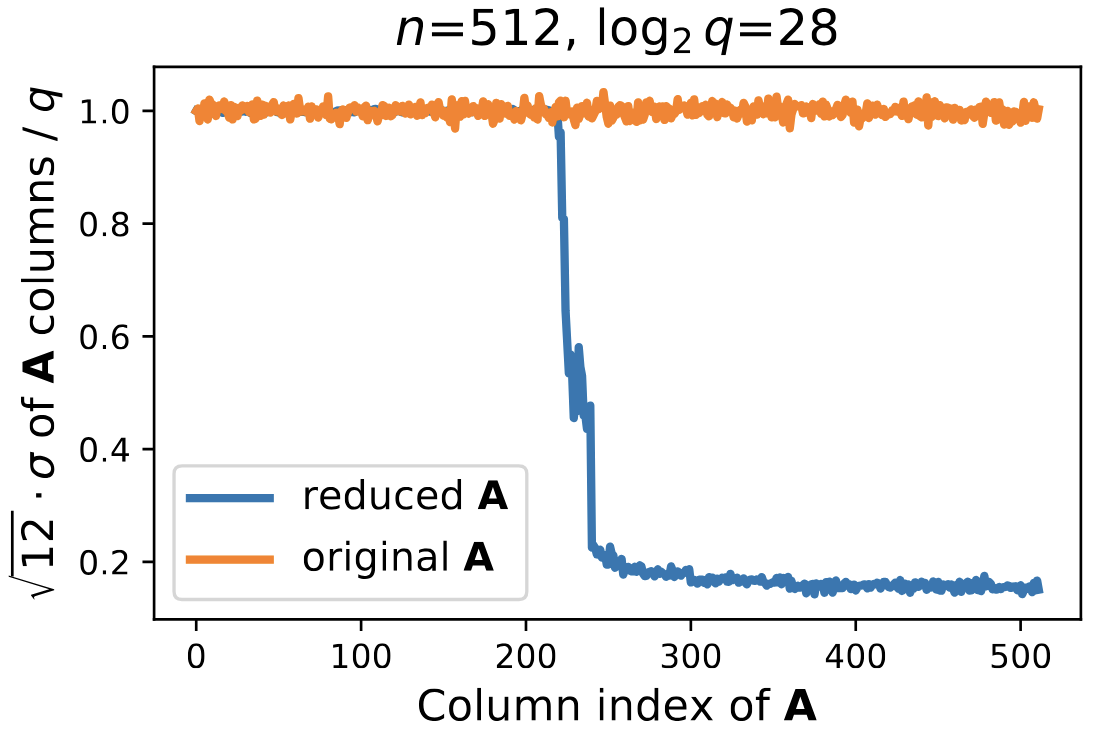
\includegraphics[width=\textwidth]{512-28.png}};
            \begin{scope}[x={(image.south east)}, y={(image.north west)}]
                % Cruel region (green frame)
                \draw[thick, green, fill=green!20, opacity=0.3] (0.18, 0.19) rectangle (0.505, 0.8);
                % Chill region (yellow frame)
                \draw[thick, yellow, fill=yellow!20, opacity=0.3] (0.510, 0.19) rectangle (0.525, 0.8);
                % Cool region (blue frame)
                \draw[thick, blue, fill=blue!20, opacity=0.3] (0.530, 0.19) rectangle (0.935, 0.8);
            \end{scope}
        \end{tikzpicture}
        \caption{\small $n=512,\,\log_2 q=28$.}
        \label{fig:region2}
    \end{subfigure}
    \caption{\small Division of columns into \textbf{Cruel} (green), \textbf{Chill} (yellow), and \textbf{Cool} (blue) zones,
    reflecting standard deviation changes post-reduction.}
    \label{fig:annotated_regions}
\end{figure}
\end{frame}

% --------------------------------------------------------------------------
\begin{frame}{Proposed Method: Threshold-Based Zoning}
\textbf{Threshold Model:}

Let $\sigma_j$ be the standard deviation of column $j$ in the reduced matrix $\mathbf{A}'$.
Define two thresholds $T_c$ and $T_h$ such that
\[
  T_c > T_h > 0, \quad \text{(e.g., }T_c \approx 0.8\,\sigma_u,\; T_h \approx 0.3\,\sigma_u\text{).}
\]
We classify each column $j$ by:
\[
  \text{Region}(j) =
  \begin{cases}
    \mathrm{Cruel} & \text{if } \sigma_j \ge T_c, \\
    \mathrm{Chill} & \text{if } T_h \;\le\;\sigma_j < T_c, \\
    \mathrm{Cool}  & \text{if } \sigma_j < T_h.
  \end{cases}
\]

\textbf{Why This Works:}
\begin{itemize}
  \item \(\sigma_j \approx q/\sqrt{12}\) $\rightarrow$ treat as Cruel, requiring heavy enumeration.
  \item \(\sigma_j \ll q/\sqrt{12}\) $\rightarrow$ treat as Cool, a small variance for easy per-bit flips.
  \item \(\sigma_j\) in-between $\rightarrow$ use a \emph{more refined} partial approach.
\end{itemize}
\end{frame}

% --------------------------------------------------------------------------
\begin{frame}[fragile]{Pseudocode: Multi-Zone Column Recovery}
\small
\textbf{Objective:} Merge brute force for Cruel bits, partial advanced method for Chill bits, and basic flips for Cool bits.

\begin{algorithmic}
\Procedure{MultiZoneRecovery}{$\mathbf{A}, \mathbf{b}, T_c, T_h$}
  \State $\text{zones} \gets \{\}$ \Comment{Cruel, Chill, Cool region indices}
  \For{$j = 0 \to n-1$}
    \State $\sigma_j \gets \mathrm{StdDev}(\mathbf{A}_{*,j})$ \Comment{post-reduction}
    \If {$\sigma_j \ge T_c$}
      \State $\text{zones}[\mathrm{Cruel}] \gets \text{zones}[\mathrm{Cruel}] \cup \{j\}$
    \ElsIf {$\sigma_j \ge T_h$}
      \State $\text{zones}[\mathrm{Chill}] \gets \text{zones}[\mathrm{Chill}] \cup \{j\}$
    \Else
      \State $\text{zones}[\mathrm{Cool}] \gets \text{zones}[\mathrm{Cool}] \cup \{j\}$
    \EndIf
  \EndFor

  \State $\mathbf{s}_{\mathrm{cruel}} \gets \mathrm{BruteForce}(\mathbf{A}_{*,\text{zones}[\mathrm{Cruel}]}, \mathbf{b})$
  \Comment{Exhaustive or hybrid search on cruel bits.}

  \State $\mathbf{s}_{\mathrm{cool}} \gets \mathrm{GreedyFlips}(\mathbf{A}_{*,\text{zones}[\mathrm{Cool}]}, \mathbf{b})$
  \Comment{Simple bit-flip approach.}

  \State $\mathbf{s}_{\mathrm{chill}} \gets \mathrm{RefinedChill}(\mathbf{A}_{*,\text{zones}[\mathrm{Chill}]}, \mathbf{b}, \mathbf{s}_{\mathrm{cruel}}, \mathbf{s}_{\mathrm{cool}})$
  \Comment{E.g., partial enumeration or advanced classifier.}

  \State \textbf{return} $\mathbf{s}_{\mathrm{cruel}} \cup \mathbf{s}_{\mathrm{chill}} \cup \mathbf{s}_{\mathrm{cool}}$
\EndProcedure
\end{algorithmic}

\textbf{Note:}
\begin{itemize}
  \item \textproc{BruteForce} may be a classic meet-in-the-middle if $|\text{zones}[\mathrm{Cruel}]|$ is large.
  \item \textproc{RefinedChill} can involve partial enumeration or an ML-based approach to handle medium-variance columns.
  \item Final correctness check can be done by verifying residual distribution on entire $\mathbf{A} \cdot \mathbf{s}^* - \mathbf{b}$.
\end{itemize}
\end{frame}

% --------------------------------------------------------------------------
\begin{frame}{Benefits and Challenges}
\textbf{Pros:}
\begin{itemize}
  \item Avoid over-enumerating columns that are ``almost cool'' but not entirely.
  \item Possibly reduce sample usage vs.\ forcing the entire slope region into a one-bit flip approach with large noise.
  \item Straightforward to implement if we define thresholds $T_c, T_h$ carefully.
\end{itemize}

\textbf{Cons / Open Questions:}
\begin{itemize}
  \item Choosing thresholds is somewhat heuristic. Slope detection or derivative-based methods might be more precise.
  \item \textproc{RefinedChill} approach must be robust: a single misclassification can invalidate the overall guess.
  \item If the slope is wide, partial enumeration might still be too big, requiring further sub-lattice re-reductions or advanced pruning.
\end{itemize}

\textbf{Future Steps:}
\begin{itemize}
  \item Experiment with different $\omega$ (penalty) to see how the slope changes in dimension $n$.
  \item Compare real run times vs.\ a single uniform approach (pure brute force or pure greedy).
  \item Investigate synergy with ring-based rotation if using RLWE (2-power cyclotomic).
\end{itemize}
\end{frame}

% ----------------------------------------------------------------------------
\begin{frame}{References}
  \footnotesize
  \begin{thebibliography}{9}
    \bibitem{regev}
    O. Regev. \emph{On Lattices, Learning with Errors, Random Linear Codes, and Cryptography.} J. ACM 51(6), 2005.

    \bibitem{concrete_results}
    Niklas N., ...
    \emph{The Cool and the Cruel: Separating Hard Parts of LWE Secrets., https://eprint.iacr.org/2024/443.pdf}
    (ArXiv, 2024).
    
    \bibitem{someRef2}
    Albrecht et al. \emph{Estimate all the LWE, NTRU schemes.  https://eprint.iacr.org/2018/331} (2018).

    \bibitem{BKZ2ref}
    Chen, Y., Nguyen, P. Q.,
    \emph{BKZ 2.0: Better Lattice Security Estimates}.
    Lecture Notes in Computer Science, 2011.

    \bibitem{FlatterRef}
    Ryan, K., Heninger, N.
    \emph{Fast practical lattice reduction through iterated compression.}
    Annual International Cryptology Conference. Springer, 2023.

    \bibitem{PolishRef}
    Charton, F., Lauter, K., Li, C., Tygert, M.
    \emph{An efficient algorithm for integer lattice reduction. SIAM Journal on Matrix Analysis and Applications}
    (2024).

    \bibitem{SALSAref}
    Gama, N., Ducas, L. et al.,
    \emph{On SALSA Picante ML Attack Method. https://eprint.iacr.org/2023/340} (2023).
    % Add more references as needed
  \end{thebibliography}
\end{frame}

% ----------------------------------------------------------------------------
\end{document}
